%%
%% A Metamodel for AI-Agent Telemetry: Assessing Diagnostic Performance
%% Target venue: MDE Intelligence 2026 (co-located with MODELS 2026)
%% Format: 5-page Extended Abstract
%%

\documentclass[sigconf,nonacm]{acmart}

\setcopyright{none}
\settopmatter{printacmref=false}
\makeatletter
\@ifundefined{footnotetextcopyrightpermission}{}{%
  \renewcommand\footnotetextcopyrightpermission[1]{}%
}
\makeatother
\pagestyle{plain}

\usepackage{listings}
\usepackage{xcolor}
\usepackage{booktabs}
\usepackage{enumitem}
\usepackage{url}
\usepackage{graphicx}
\usepackage{tikz}
\usetikzlibrary{positioning,arrows.meta,shapes.geometric,calc,fit}
\usepackage{seqsplit}
\usepackage{amssymb}

\hyphenation{Open-Tele-metry Open-Inference meta-model meta-models meta-modeling de-le-ga-tion co-or-di-na-tion AgentTelemetry agent-telemetry guard-rail con-form-ance ex-pres-siv-i-ty}

\setlength{\emergencystretch}{3em}

\lstset{
  basicstyle=\ttfamily\footnotesize,
  keywordstyle=\color{blue!70!black}\bfseries,
  commentstyle=\color{green!50!black}\itshape,
  stringstyle=\color{red!60!black},
  showstringspaces=false,
  breaklines=true,
  breakatwhitespace=true,
  frame=single,
  framesep=3pt,
  xleftmargin=4pt,
  xrightmargin=2pt,
  aboveskip=4pt,
  belowskip=4pt,
  columns=flexible,
}

\lstdefinelanguage{OCL}{
  morekeywords={context,inv,pre,post,let,in,if,then,else,endif,
    self,implies,and,or,not,forAll,exists,select,collect,size,
    includes,oclIsKindOf,oclIsUndefined,oclAsType,Set,Bag,Sequence,Tuple,
    String,Integer,Boolean,SpanKind},
  sensitive=true,
  morecomment=[l]{--},
  morestring=[b]'
}

\begin{document}

\title{A Metamodel for AI-Agent Telemetry:\\Assessing Diagnostic Performance}

\author{Krishna Chaitanya Balusu}
\affiliation{%
  \institution{Independent Researcher}
  \city{San Francisco}
  \state{CA}
  \country{United States}
}
\email{krishna.balusu@outlook.com}

\begin{abstract}
Autonomous AI agents built on large language models are entering production, but the observability infrastructure that monitors them remains constrained by legacy metamodels. Generic OpenTelemetry was designed for request--response microservices; the AI-specific conventions OpenTelemetry GenAI and OpenInference introduce typed agent and tool entities but lack typed sub-operations for delegation topology, planning, reasoning, memory, and constrained guardrail outcomes. We present a Domain-Specific Metamodel (DSM) for AI-agent telemetry: an Ecore abstract syntax with nine semantic span kinds, six OCL well-formedness invariants, and a W3C-compatible context propagation profile. Aligning with the workshop's special theme of assessing MDE performance, we conduct a constructive evaluation of observability \emph{expressivity} on a small synthetic benchmark of fourteen agent-specific fault classes (thirteen mapped onto the MAST taxonomy of Cemri et al.) across six telemetry conditions, seven agent frameworks, and six mocked foundation models; the foundation-model dimension contributes no independent variance, so the effective evaluation is a deterministic coverage matrix over fault, framework, and telemetry schema. Vanilla OTel, OTel GenAI, and OpenInference all converge to FDR 0.429 \emph{under typed-only comparison}; the DSM averages 0.612 across all seven adapters (FPR 0.071, due to the \texttt{infinite\_loop} detector misfiring on legitimately repeated CrewAI tool calls) and reaches a constructive upper bound of 1.000 on the conformance-complete reference adapter. The result is typed-metamodel \emph{expressivity}, not production diagnostic performance. The artifact (Ecore, OCL, fault$\rightarrow$element table, coverage matrix, MAST mapping, pinned environment) is released with the paper.
\end{abstract}

\maketitle

\section{Introduction}

Autonomous agents built on large language models (LLMs) are no longer toy projects; they execute production workflows in customer support, code generation, and incident response \cite{wu2023autogen,langchain2023,crewai2023}. Unlike traditional software, agents operate through stochastic loops of \emph{planning}, \emph{tool execution}, \emph{reasoning}, and \emph{delegation}. As they enter production, observability has become critical, and a growing body of evidence shows that multi-agent failures are dominated by \emph{agent-specific} pathologies (system design, inter-agent misalignment, task verification) rather than the network errors that dominate microservice incidents \cite{cemri2025multiagent}.

Observability is fundamentally a metamodeling problem \cite{atkinson2003mdd,bezivin2005unification,brambilla2017mde}. A telemetry stack is a metamodel that fixes \emph{what} execution data is captured, \emph{how} it is categorized, and \emph{how} disparate traces are graphed. The de-facto standard, OpenTelemetry (OTel), defines a metamodel for distributed traces whose abstract syntax centers on \texttt{Span} entities classified by a small \texttt{SpanKind} enumeration (\texttt{CLIENT}, \texttt{SERVER}, \texttt{INTERNAL}, \texttt{PRODUCER}, \texttt{CONSUMER}). It was designed for request--response microservices.

Two AI-specific conventions extend OTel: OTel GenAI \cite{opentelemetry-genai} introduces nine operation names that include \texttt{chat}, \texttt{create\_agent}, \texttt{invoke\_agent}, \texttt{invoke\_workflow}, \texttt{execute\_tool}, and \texttt{retrieval}; OpenInference \cite{openinference2024} introduces ten typed span kinds spanning LLM, embedding, chain, retriever, reranker, tool, agent, guardrail, evaluator, and prompt. Both narrow the gap relative to vanilla OTel. Neither, however, provides typed sub-operations for the cognitive and coordination phases that distinguish agent workflows: \emph{planning}, \emph{reasoning}, peer-agent \emph{delegation} with typed source/target identifiers, \emph{memory} operations, and constrained guardrail outcomes. In both, ``invoke an agent'' or ``invoke a workflow'' is an opaque LLM-framed wrapper.

We address this gap by applying Model-Driven Engineering principles to the observability schema for autonomous agents. Our contributions are:

\begingroup\sloppy
\begin{enumerate}[label=(C\arabic*),leftmargin=*]
\item A \textbf{Domain-Specific Metamodel} (DSM) defined as an Ecore-style abstract syntax (Fig.~\ref{fig:metamodel}) with nine semantic \texttt{SpanKind} entities, six OCL well-formedness invariants (Listing~\ref{lst:ocl}), and a W3C-compatible context propagation profile (\S\ref{sec:dsm}).
\item A \textbf{constructive performance assessment} of the DSM against generic OTel, OTel GenAI (with the current \texttt{retrieval}, \texttt{create\_agent}, and \texttt{invoke\_agent} operations), and OpenInference (six of ten typed kinds exercised) on fourteen agent-specific fault classes mapped onto MAST \cite{cemri2025multiagent}, over 3{,}528 fault-injection runs plus 252 fault-free controls (\S\ref{sec:assessment}). All numbers are reproduced from the artifact.
\item A \textbf{conformance analysis} (\S\ref{sec:conformance}) that separates \emph{metamodel expressivity} (decisive: only the DSM can express the eight coordination/cognitive/policy faults) from \emph{adapter conformance} (with a 3/9-to-7/9 coverage spread across third-party frameworks), and motivates conformance-driven adapter generation as the next research direction.
\end{enumerate}
\endgroup

\section{Related Work}
\label{sec:related}

\textbf{MDE for AI.} The MDE Intelligence series has applied MDE to AI artifacts: instance model generation from LLMs \cite{pan2025instance}, syntactic-validity guarantees via grammar masking \cite{netz2024grammarmask}, DSML construction with LLM assistance \cite{disipio2024dsml}, conformance preservation under LLM-driven model edits \cite{netz2025unintended}, and modeling AI-driven workflows \cite{sousa2025aiworkflows}. Our work continues this MDE-for-AI direction but targets the \emph{runtime} artifact (telemetry traces) rather than design-time artifacts. C\'amara et al.\ \cite{camara2023assessment} evaluate generative AI on modeling tasks; we conversely apply modeling techniques to evaluate observability of AI \cite{burgueno2022editorial}.

\textbf{AI agent observability.} Three industry vocabularies compete: OpenTelemetry GenAI \cite{opentelemetry-genai} (operation-name oriented), OpenInference \cite{openinference2024} (kind-oriented; ten typed kinds including \texttt{AGENT}, \texttt{GUARDRAIL}, \texttt{RETRIEVER}, \texttt{TOOL}), and proprietary stacks (LangSmith, Phoenix). The closest to our DSM is OpenInference, which lifts \texttt{AGENT} and \texttt{GUARDRAIL} to typed spans; however, its \texttt{AGENT} is a coarse wrapper without typed sub-operations for planning, reasoning, delegation, or memory, and its \texttt{GUARDRAIL} carries free-form attributes rather than a constrained outcome. Our DSM splits \texttt{AGENT} into seven sub-kinds plus typed memory, gives \texttt{Delegation} explicit source/target identifiers, and binds the whole with OCL invariants. \emph{We benchmark all three baselines empirically} (\S\ref{sec:assessment}).

\textbf{Telemetry metamodeling and runtime models.} OpenTelemetry Schema URLs / Schema Files version a telemetry vocabulary as a first-class artifact; DMTF's CIM \cite{dmtf-cim} does the same for system monitoring. The MDE community has long studied \emph{models@runtime} \cite{blair2009runtime} and model-based monitoring; production agent observability stacks (LangSmith, Arize Phoenix, OpenInference) are essentially industry instances with implicit (untyped) trace metamodels. We make the trace metamodel explicit, typed, and OCL-constrained.

\textbf{Metamodel evaluation.} Bork et al.\ \cite{bork2020specification} survey modeling-language specification techniques and call for systematic evaluation. Whittle et al.\ \cite{whittle2014state} document the gap between MDE practice and MDE evaluation. Our use of FDR as a constructive expressivity probe is a step toward such evaluation for the observability sub-domain.

\section{The Semantic Gap}
\label{sec:gap}

Consider the lifecycle of a single agent task: receive a user prompt, decompose it into a plan, query an LLM to reason over the plan, invoke a code-interpreter tool, delegate a sub-task to a researcher agent, retrieve grounded context, and pass the final output through a safety guardrail. Table~\ref{tab:gap} contrasts how four observability metamodels --- generic OTel, OTel GenAI, OpenInference, and our DSM --- categorize each step.

\begin{table}[h]
\centering
\caption{Semantic information loss across observability metamodels.}
\label{tab:gap}
\footnotesize
\begin{tabular}{p{1.55cm} p{1.05cm} p{1.25cm} p{1.25cm} p{1.4cm}}
\toprule
\textbf{Operation} & \textbf{V-OTel} & \textbf{OTel GenAI} & \textbf{Open\-Inference} & \textbf{DSM (ours)} \\
\midrule
LLM call        & \texttt{CLIENT}   & \texttt{chat}            & \texttt{LLM}       & \texttt{LLM\_CALL} \\
Tool exec.      & \texttt{CLIENT}   & \texttt{execute\_tool}   & \texttt{TOOL}      & \texttt{TOOL\_CALL} \\
Plan gen.       & \texttt{INTERNAL} & \texttt{chat}            & \texttt{CHAIN}     & \texttt{PLANNING} \\
Reasoning step  & \texttt{INTERNAL} & \texttt{chat}            & \texttt{CHAIN}     & \texttt{REASONING} \\
Delegation      & \texttt{CLIENT}   & \texttt{invoke\_agent}\textsuperscript{$\dagger$} & \texttt{AGENT}\textsuperscript{$\dagger$} & \texttt{DELEGATION} \\
RAG retrieval   & \texttt{CLIENT}   & \texttt{retrieval}       & \texttt{RETRIEVER} & \texttt{RETRIEVAL} \\
Guardrail       & \texttt{INTERNAL} & --                       & \texttt{GUARDRAIL}\textsuperscript{$\ddagger$} & \texttt{GUARD\_RAIL} \\
Memory r/w      & \texttt{INTERNAL} & --                       & --                 & \texttt{MEMORY} \\
Agent lifecycle & --                & \texttt{create\_agent}   & \texttt{AGENT}     & \texttt{AGENT} \\
\bottomrule
\end{tabular}
\\
\raggedright\textsuperscript{$\dagger$}\,Opaque wrapper without typed parent/target identity.\quad\textsuperscript{$\ddagger$}\,Free-form attributes; no constrained \texttt{pass}/\texttt{fail}/\texttt{warn} outcome.
\end{table}

\section{A Domain-Specific Metamodel for AI Agent Observability}
\label{sec:dsm}

\sloppy
We define the DSM as a metamodel conforming to MOF \cite{omg-mof}, expressed in Ecore \cite{steinberg2008emf}; the machine-readable metamodel and OCL invariants are released with the artifact (\texttt{agenttelemetry.\allowbreak ecore}, \texttt{agenttelemetry.\allowbreak ocl}). Figure~\ref{fig:metamodel} gives the abstract syntax. The root container is \texttt{Trace}, which owns \texttt{AgentSpan} instances. \texttt{AgentSpan} is abstract; nine concrete subclasses cover the agent operations (one per \texttt{SpanKind}). Each \texttt{AgentSpan} carries \texttt{Attribute}s, \texttt{BaggageEntry}s, a \texttt{parentId}, and an \texttt{agentId}. The \texttt{Delegation} subclass exposes \texttt{sourceAgent} and \texttt{targetAgent} as Ecore-derived fields (\texttt{derived="true"}) that project the underlying generic \texttt{Attribute} entries with keys \texttt{delegation.\seqsplit{source\_agent}} and \texttt{delegation.\seqsplit{target\_agent}}; the OCL invariants read those same generic keys, so the structural fields and OCL operate on a single source of truth. The \texttt{kind} discriminator on \texttt{AgentSpan} is itself derived: a GenModel \texttt{EAnnotation} encodes the rule that \texttt{kind} equals the \texttt{SpanKind} literal of the concrete subclass.
\fussy

\begin{figure}[h]
\centering
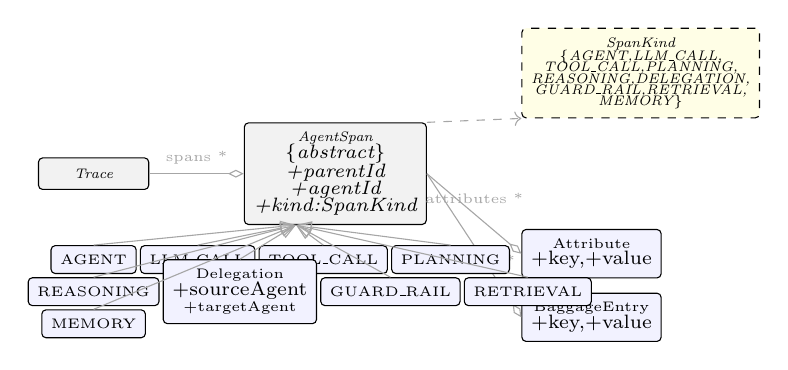
\begin{tikzpicture}[
  font=\tiny,
  every node/.style={align=center},
  cls/.style={draw, rounded corners=1.5pt, minimum width=1.05cm, minimum height=0.32cm, fill=blue!5},
  abs/.style={draw, rounded corners=1.5pt, minimum width=1.4cm, minimum height=0.4cm, fill=gray!10, font=\tiny\itshape},
  enum/.style={draw, dashed, rounded corners=1.5pt, minimum width=1.4cm, minimum height=0.4cm, fill=yellow!10, font=\tiny\itshape},
  comp/.style={-{Diamond[length=2mm,open]}, gray!70},
  inh/.style={-{Triangle[length=2mm,open]}, gray!70}
]
\node[abs] (trace) {Trace};
\node[abs, right=1.2cm of trace] (span) {AgentSpan\\[-1pt]\scriptsize\itshape\{abstract\}\\[-1pt]\scriptsize+parentId\\[-1pt]\scriptsize+agentId\\[-1pt]\scriptsize+kind:SpanKind};
\node[enum, above right=0.05cm and 1.2cm of span] (kind) {SpanKind\\[-1pt]\{AGENT,LLM\_CALL,\\[-2pt]TOOL\_CALL,PLANNING,\\[-2pt]REASONING,DELEGATION,\\[-2pt]GUARD\_RAIL,RETRIEVAL,\\[-2pt]MEMORY\}};
\node[cls, below right=0.05cm and 1.2cm of span] (attr) {Attribute\\\scriptsize+key,+value};
\node[cls, below=0.18cm of attr] (bag) {BaggageEntry\\\scriptsize+key,+value};

\draw[comp] (trace.east) -- node[above,font=\tiny]{spans *} (span.west);
\draw[comp] (span.east) -- node[above,font=\tiny]{attributes *} (attr.west);
\draw[comp] (span.east) -- node[below,font=\tiny]{baggage *} (bag.west);
\draw[->,gray!70,dashed] (span.north east) -- (kind.south west);

\node[cls, below=0.7cm of trace] (a) {AGENT};
\node[cls, right=0.04cm of a] (l) {LLM\_CALL};
\node[cls, right=0.04cm of l] (t) {TOOL\_CALL};
\node[cls, right=0.04cm of t] (p) {PLANNING};
\node[cls, below=0.04cm of a] (r) {REASONING};
\node[cls, right=0.04cm of r] (d) {Delegation\\\scriptsize+sourceAgent\\+targetAgent};
\node[cls, right=0.04cm of d] (g) {GUARD\_RAIL};
\node[cls, right=0.04cm of g] (rt) {RETRIEVAL};
\node[cls, below=0.04cm of r] (m) {MEMORY};

\foreach \n in {a,l,t,p,r,d,g,rt,m} \draw[inh] (\n.north) -- ($(span.south) + (-0.5,0)$);
\end{tikzpicture}
\Description{Ecore-style class diagram. A Trace class composes zero-or-more AgentSpan instances. AgentSpan is abstract and is specialized into nine concrete subclasses: AGENT, LLM_CALL, TOOL_CALL, PLANNING, REASONING, DELEGATION, GUARD_RAIL, RETRIEVAL, MEMORY. Each AgentSpan composes zero-or-more Attribute and BaggageEntry instances and carries parentId, agentId, and a redundant kind:SpanKind discriminator. The Delegation subclass adds typed sourceAgent and targetAgent attributes. A SpanKind enumeration with the same nine literals is shown alongside.}
\caption{Ecore-style abstract syntax of the DSM.}
\label{fig:metamodel}
\end{figure}

\subsection{Well-formedness constraints}

Six OCL invariants \cite{omg-ocl} (Listing~\ref{lst:ocl}) accompany the metamodel. Five cover one distinct fault category each (two for coordination, one for topology, one for execution, one for policy); the sixth, \texttt{KindMatchesSubtype}, ties the redundant \texttt{kind} discriminator to the concrete subclass, closing the discriminator-vs-subclass loophole.

\begin{lstlisting}[language=OCL,caption={OCL well-formedness constraints on the DSM (released as \texttt{agenttelemetry.ocl}).},label={lst:ocl}]
context Trace inv RootIsAgent:
  self.spans
    ->select(s | s.parentId.oclIsUndefined())
    ->forAll(s | s.kind = SpanKind::AGENT)

context AgentSpan inv DelegationCarriesIdentity:
  self.kind = SpanKind::DELEGATION implies (
    self.attributes->exists(a |
      a.key = 'delegation.source_agent') and
    self.attributes->exists(a |
      a.key = 'delegation.target_agent'))

context Trace inv NoCircularDelegation:
  -- pairwise (2-cycle) check; longer-cycle SCC
  -- handled by the runtime conformance checker.
  let edges =
    self.spans->select(s | s.kind = SpanKind::DELEGATION)
      ->collect(s | Tuple {
          src = s.attributes->select(a |
                  a.key='delegation.source_agent')
                  ->first().value,
          tgt = s.attributes->select(a |
                  a.key='delegation.target_agent')
                  ->first().value }) in
  edges->forAll(e1 | edges->forAll(e2 |
    not (e1.src = e2.tgt and e1.tgt = e2.src)))

context AgentSpan inv CostMetricsRequired:
  self.kind = SpanKind::LLM_CALL implies (
    self.attributes->exists(a | a.key='llm.input_tokens')  and
    self.attributes->exists(a | a.key='llm.output_tokens') and
    self.attributes->exists(a | a.key='llm.cost'))

context AgentSpan inv GuardRailResultIsExplicit:
  self.kind = SpanKind::GUARD_RAIL implies
    self.attributes->exists(a |
      a.key = 'guardrail.result' and
      Set{'pass','fail','warn','bypass'}->includes(
        a.value.oclAsType(String)))

context AgentSpan inv KindMatchesSubtype:
  -- closes the discriminator-vs-subclass loophole.
  Sequence{Agent,LlmCall,ToolCall,Planning,Reasoning,
           Delegation,GuardRail,Retrieval,Memory}
    ->forAll(c | self.oclIsKindOf(c) implies
                 self.kind = SpanKind::valueOf(c.name))
\end{lstlisting}
\Description{Six OCL well-formedness invariants over the DSM: RootIsAgent, DelegationCarriesIdentity, NoCircularDelegation, CostMetricsRequired, GuardRailResultIsExplicit, and KindMatchesSubtype tying the kind discriminator to the concrete subclass.}

\subsection{Inter-agent context propagation}

The DSM uses two complementary identity mechanisms. Within a trace, topology is captured by typed source/target attributes on \texttt{Delegation} spans (\texttt{delegation.\seqsplit{source\_agent}} / \texttt{delegation.\seqsplit{target\_agent}}; see Listing~\ref{lst:ocl}). Across processes, the DSM extends W3C Trace Context \cite{w3c-trace-context} and Baggage \cite{w3c-baggage} with two semantic baggage keys that propagate agent identity across HTTP and message-queue boundaries. The \texttt{NoCircularDelegation} invariant and the \texttt{circular\_delegation} detector both read the in-trace pair; the runtime conformance checker validates that the baggage keys appear on every cross-process span downstream of a \texttt{Delegation}.

\section{Assessing Metamodel Performance}
\label{sec:assessment}

In MDE, the performance of an observability metamodel is its \emph{diagnostic utility}: how effectively does the metamodel let an automated rule decide whether a given trace contains a fault? We assess the DSM using Fault Detection Rate (FDR) paired with False-Positive Rate (FPR). We frame this as a \emph{constructive evaluation of observability expressivity}: we measure whether each metamodel can in principle support detection of each fault class on the seven adapter+app pairs we built; we do not claim production diagnostic validation on independent workloads.

\subsection{Methodology}

\paragraph{Fault taxonomy.}
We constructed a taxonomy of fourteen agent-specific fault types and mapped each onto the multi-agent failure taxonomy (MAST) of Cemri et al.\ \cite{cemri2025multiagent}, whose three categories are \emph{system design issues}, \emph{inter-agent misalignment}, and \emph{task verification}. Thirteen of fourteen faults map to MAST modes (artifact: \texttt{mast\_}\-\texttt{mapping.md}); \texttt{cost\_explosion} is our addition. Of MAST's fourteen modes (FM-1.1 through FM-3.3), our taxonomy covers twelve distinct modes; the two unmapped modes --- FM-1.2 (Disobey Role Specification) and FM-2.2 (Fail to Ask for Clarification) --- are not observable from runtime telemetry alone. Six of the fourteen faults surface from generic OTel attributes alone (the ``easy six''); the remaining eight require typed agent-specific spans (the ``hard eight'').

\paragraph{Conditions.} We test six telemetry conditions: (a)~\textbf{No Telemetry} (control); (b)~\textbf{Vanilla OTel}; (c)~\textbf{OTel GenAI} (current spec: \texttt{chat}, \texttt{create\_agent}, \texttt{invoke\_agent}, \texttt{execute\_tool}, \texttt{retrieval}, \texttt{embeddings}); (d)~\textbf{OpenInference} (typed kinds \texttt{AGENT}, \texttt{LLM}, \texttt{TOOL}, \texttt{CHAIN}, \texttt{RETRIEVER}, \texttt{GUARDRAIL}); (e)~\textbf{DSM (Metadata)} (nine kinds, prompts/completions redacted); (f)~\textbf{DSM (Full)} (nine kinds, full payload).

\paragraph{Experimental matrix.} We run all 14 faults $\times$ 6 conditions $\times$ 7 frameworks $\times$ 6 mocked foundation models = 3{,}528 fault-injection runs, plus 6 $\times$ 7 $\times$ 6 = 252 fault-free control runs (for FPR), all on a deterministic seed. The model dimension does not contribute additional fault-detection variance under deterministic mocks; we retain it because it varies the cost-per-token magnitudes that drive the \texttt{cost\_explosion} detector.

\paragraph{Detector.} For each (condition, fault) pair we hand-coded a deterministic Python predicate over exported spans (one branch per fault, four banks for vanilla / GenAI / OpenInference / DSM). Predicates use only what the metamodel exposes. For instance, the DSM \texttt{circular\_delegation} detector is one line --- find a pair of \texttt{DELEGATION} spans whose \emph{(src,tgt)} reverses --- because the metamodel makes the topology explicit. The same predicate is impossible to write under the three baselines because none exposes typed \texttt{(agent\_id, target\_id)} on a typed delegation span. A trace is positive iff the predicate fires.

\paragraph{Fault $\rightarrow$ metamodel-element mapping.}
Table~\ref{tab:faultmap} gives the exact DSM element, OCL invariant (where applicable), and detector attribute that each fault relies on. Faults whose required element is absent in a baseline metamodel are unobservable in that baseline by construction.

\begin{table}[h]
\centering
\caption{Each fault $\rightarrow$ required DSM element, OCL invariant (if any), and detector attribute. \emph{Easy} = surfaces from generic LLM/tool attributes; \emph{Hard} = requires agent-specific typed spans.}
\label{tab:faultmap}
\scriptsize
\setlength{\tabcolsep}{2pt}
\begin{tabular}{p{1.55cm} p{1.5cm} p{1.4cm} p{2.4cm}}
\toprule
\textbf{Fault} & \textbf{DSM element} & \textbf{OCL inv.} & \textbf{Detector attribute} \\
\midrule
\multicolumn{4}{l}{\emph{Easy six (detectable by all telemetry conditions):}}\\
\texttt{wrong\_tool}        & \texttt{TOOL\_CALL}   & --                          & \texttt{tool.name} \\
\texttt{infinite\_loop}     & \texttt{TOOL\_CALL}   & --                          & repeated \texttt{tool.name} \\
\texttt{tool\_failure}      & \texttt{TOOL\_CALL}   & --                          & OTel \texttt{ERROR} \\
\texttt{timeout}            & any                   & --                          & \texttt{ERROR}+``timeout'' \\
\texttt{context\_overflow}  & \texttt{LLM\_CALL}    & \texttt{CostMetrics}        & \texttt{llm.input\_tokens} \\
\texttt{cost\_explosion}    & \texttt{LLM\_CALL}    & \texttt{CostMetrics}        & sum(\texttt{llm.cost}) \\
\midrule
\multicolumn{4}{l}{\emph{Hard eight (detectable only with DSM-conformant traces):}}\\
\texttt{circular\_deleg.}   & \texttt{DELEGATION}   & \texttt{NoCircular}         & \texttt{delegation.\{src,tgt\}\_agent} \\
\texttt{hallucination}      & \texttt{LLM\_CALL}, \texttt{RETRIEVAL} & --        & no \texttt{RETRIEVAL} sibling \\
\texttt{stale\_retrieval}   & \texttt{RETRIEVAL}    & --                          & \texttt{retrieval.\seqsplit{staleness\_seconds}} \\
\texttt{guardrail\_byp.}    & \texttt{GUARD\_RAIL}  & \texttt{GuardRail}          & \texttt{guardrail.result} \\
\texttt{planning\_failure}  & \texttt{PLANNING}     & --                          & \texttt{planning.step\_count} \\
\texttt{reasoning\_loop}    & \texttt{REASONING}    & --                          & \texttt{reasoning.chain} \\
\texttt{agent\_misroute}    & \texttt{AGENT}, \texttt{DELEG.} & \texttt{Deleg.Id.} & \texttt{agent.misrouted} \\
\texttt{memory\_corrupt.}   & \texttt{MEMORY}       & --                          & \texttt{memory.corrupted} \\
\bottomrule
\end{tabular}
\end{table}

\subsection{Results}

\begin{table}[h]
\centering
\caption{Aggregate FDR (over 3{,}528 fault-injection runs) and FPR (over 252 fault-free runs).}
\label{tab:fdr}
\small
\begin{tabular}{p{2.6cm}ccc}
\toprule
\textbf{Condition} & \textbf{FDR} & \textbf{FPR} & \textbf{@\,FDR=1} \\
\midrule
No Telemetry          & 0.000 & 0.000 & 0/14 \\
Vanilla OTel          & 0.429 & 0.000 & 6/14 \\
OTel GenAI (current spec) & 0.429 & 0.000 & 6/14 \\
OpenInference         & 0.429 & 0.000 & 6/14 \\
DSM (Metadata)        & 0.612 & 0.071 & 7/14 \\
DSM (Full)            & 0.612 & 0.071 & 7/14 \\
\midrule
\textit{DSM, ref.\ adapter (upper bound)} & \textbf{1.000} & \textbf{0.000} & \textbf{14/14} \\
\bottomrule
\end{tabular}
\end{table}

DSM (Metadata) and DSM (Full) are identical because every detector operates on typed structure and metadata attributes, never on payloads --- payload redaction is FDR-neutral, an explicit privacy benefit of the design. The DSM FPR of 0.071 originates from three CrewAI fault-free runs (out of 42 per condition; reproducible with the artifact's \texttt{compute\_fpr.py}) on which the \texttt{infinite\_loop} detector misfires: the CrewAI multi-agent workload legitimately invokes the same \texttt{tool-calculator} three times across writer turns, exceeding the detector's count$\geq$3 threshold. We treat this as a real false-positive of the threshold-based detector against a non-fault repeated-tool pattern, not a metamodel defect; tightening the detector to require both repetition \emph{and} no monotonic state progression is straightforward future work.

\textbf{Scope: standardized typed semantics.} The \texttt{otel\_genai} and \texttt{openinference} detectors exploit only the typed kinds and standardized attributes each spec defines. The OpenInference benchmark app does emit free-form delegation attributes (\texttt{delegation.\seqsplit{source\_agent}}, \texttt{delegation.\seqsplit{target\_agent}}) on its \texttt{AGENT} child span; we exclude these from the OpenInference detector because they are not part of the OpenInference typed model. The comparison is between standardized typed semantics; a custom-attribute baseline would be isomorphic to a partial DSM and is left to future work.

\textbf{Finding 1: All three baselines converge.} Vanilla OTel, the corrected OTel GenAI, and OpenInference all reach 0.429. Each detects the same six faults --- those surfacing as LLM-call or tool-call attributes. Despite GenAI providing \texttt{invoke\_agent} and OpenInference providing \texttt{AGENT}/\texttt{GUARDRAIL}, none can detect any of the eight coordination/cognitive/policy faults: \texttt{invoke\_agent} carries no source/target identifier, OpenInference \texttt{AGENT} is a coarse wrapper, and \texttt{GUARDRAIL} carries no constrained outcome. In this benchmark, under typed-only comparison, typed agent kinds without typed sub-operations close none of the diagnostic gap.

\textbf{Finding 2: Metamodel expressivity is necessary but not sufficient.} The DSM is the only metamodel that \emph{can} express the failing eight fault classes. On the reference \texttt{custom\_agent} (Listing~\ref{lst:ocl}-conformant), the DSM reaches FDR = 1.000 across all 14 faults. Aggregated across all seven adapter+app pairs, the DSM averages 0.612: the six easy faults at 1.000 plus heterogeneous partial credit on the eight hard faults (Table~\ref{fig:perfault}). The 1.000 result is a constructive upper bound (the reference adapter and the detectors share authorship), demonstrating expressivity rather than independent empirical validation.

\textbf{Finding 3: The remaining gap is a per-app conformance problem.} Per-app DSM coverage in the seven benchmark apps spans 3/9 to 9/9 (artifact: \texttt{coverage\_matrix.md}): \texttt{custom\_}\-\texttt{agent} 9/9, \texttt{llamaindex\_}\-\texttt{agent} 7/9, \texttt{langchain\_}\-\texttt{rag} 6/9, \texttt{autogen\_}\-\texttt{group} 5/9, \texttt{crewai\_}\-\texttt{team} 4/9, \texttt{anthropic\_}\-\texttt{sdk} and \texttt{openai\_}\-\texttt{sdk} 3/9. All seven emit typed \texttt{DELEGATION} when the workload requires it, so \texttt{circular\_}\-\texttt{delegation} reaches FDR = 1.000 across all apps. Only \texttt{custom\_}\-\texttt{agent} emits \texttt{GUARD\_RAIL} and \texttt{MEMORY} with conformant attributes (and \texttt{retrieval.staleness\_seconds}) --- the six remaining hard faults collapse to FDR = 0.143 (1/7). The exception is \texttt{hallucination}: five of seven apps detect it (FDR = 0.71), because the no-grounding heuristic fires on a long \texttt{LLM\_CALL} output without a sibling \texttt{RETRIEVAL}; LangChain and LlamaIndex emit non-conformant retrieval annotations under our injection that defeat the heuristic.

\begin{table}[h]
\centering
\caption{Per-fault FDR. \textbf{DSM} is the all-frameworks aggregate (0.14 = 1/7 framework conformance); \textbf{DSM*} restricts to the conformance-complete \texttt{custom\_agent} reference adapter and is reported as a constructive upper bound.}
\label{fig:perfault}
\footnotesize
\begin{tabular}{p{2.0cm} c c c c c c}
\toprule
\textbf{Fault} & \textbf{None} & \textbf{V-OT} & \textbf{GenAI} & \textbf{OI} & \textbf{DSM} & \textbf{DSM*} \\
\midrule
\texttt{wrong\_tool}        & 0.00 & 1.00 & 1.00 & 1.00 & 1.00 & 1.00 \\
\texttt{infinite\_loop}     & 0.00 & 1.00 & 1.00 & 1.00 & 1.00 & 1.00 \\
\texttt{tool\_failure}      & 0.00 & 1.00 & 1.00 & 1.00 & 1.00 & 1.00 \\
\texttt{timeout}            & 0.00 & 1.00 & 1.00 & 1.00 & 1.00 & 1.00 \\
\texttt{context\_overflow}  & 0.00 & 1.00 & 1.00 & 1.00 & 1.00 & 1.00 \\
\texttt{cost\_explosion}    & 0.00 & 1.00 & 1.00 & 1.00 & 1.00 & 1.00 \\
\midrule
\texttt{circular\_deleg.}   & 0.00 & 0.00 & 0.00 & 0.00 & 1.00 & 1.00 \\
\texttt{hallucination}      & 0.00 & 0.00 & 0.00 & 0.00 & 0.71 & 1.00 \\
\texttt{stale\_retrieval}   & 0.00 & 0.00 & 0.00 & 0.00 & 0.14 & 1.00 \\
\texttt{guardrail\_bypass}  & 0.00 & 0.00 & 0.00 & 0.00 & 0.14 & 1.00 \\
\texttt{planning\_failure}  & 0.00 & 0.00 & 0.00 & 0.00 & 0.14 & 1.00 \\
\texttt{reasoning\_loop}    & 0.00 & 0.00 & 0.00 & 0.00 & 0.14 & 1.00 \\
\texttt{agent\_misroute}    & 0.00 & 0.00 & 0.00 & 0.00 & 0.14 & 1.00 \\
\texttt{memory\_corruption} & 0.00 & 0.00 & 0.00 & 0.00 & 0.14 & 1.00 \\
\bottomrule
\end{tabular}
\end{table}

\subsection{Threats to validity}

\textbf{Construct.} FDR is a binary detection metric; it does not capture diagnostic \emph{quality}. We restrict positive signal to deterministic predicates that name the exact fault, partially mitigating this. We additionally report FPR.

\textbf{Internal (constructive bias).} The fourteen-fault taxonomy, the nine DSM kinds, the OCL invariants, the detectors, and the reference \texttt{custom\_agent} are all authored by us, so the 1.000 result is a \emph{constructive upper bound} demonstrating expressivity rather than independent empirical validation. We mitigate by mapping the fault taxonomy onto MAST and benchmarking three independent industry baselines (Vanilla OTel, OTel GenAI, OpenInference). The honest empirical claim is twofold: (a) the DSM is necessary --- no metamodel without typed coordination/cognitive/policy spans detected any of the eight hard faults --- and (b) at least one prototype adapter realizes the metamodel. We do not claim external validity beyond these synthetic benchmark scenarios; production diagnostic validation on independent third-party traces is future work.

\textbf{Statistical reporting.} All numbers are exact under deterministic mocks (single seed, fixed RNG); they are not point estimates with sampling variance. A stochastic re-evaluation under multiple seeds with 95\% CIs and real LLM endpoints is the next milestone.

\textbf{Aggregation.} Reporting an arithmetic mean over seven frameworks, several at 0.000 on the eight hard faults, can inflate the apparent score. We accordingly report both the aggregate (Table~\ref{tab:fdr}) and the per-fault breakdown (Table~\ref{fig:perfault}); the per-framework breakdown is in the artifact.

\section{Conformance and the Adapter-Generation Direction}
\label{sec:conformance}

The split between metamodel expressivity (1.000 on the conforming app) and aggregated FDR (0.612) is the actionable result. It localizes the bottleneck to a well-known MDE problem: instance conformance to a metamodel \cite{atkinson2003mdd}. Each adapter is, in MDE terms, a model-to-model transformation from framework events to DSM-conformant spans. Three follow-up directions: (i)~LLM-assisted adapter synthesis seeded by the metamodel as a target schema, e.g.\ a grammar-masked prompt \cite{netz2024grammarmask} constraining the model to emit only constructors that satisfy Listing~\ref{lst:ocl}; (ii)~runtime conformance checking that loads \texttt{agenttelemetry.ocl} into Eclipse OCL or USE and validates exported traces against all six invariants; and (iii)~a state-aware OCL constraint that distinguishes legitimate retries from pathological loops, motivated by the present CrewAI false positive.

\section{Reproducibility}
\label{sec:repro}

\begingroup\sloppy
Released as a replication artifact: the machine-readable Ecore metamodel and OCL invariants (\texttt{agenttelemetry.ecore} / \texttt{.ocl}), benchmark code, fault injectors, per-app coverage matrix, MAST mapping, an FPR script, per-run results (3{,}780 rows), and a pinned environment (\texttt{requirements.lock}, Python~3.11+; full matrix runs in $\approx$3~min on one CPU). Tables~\ref{tab:fdr} and~\ref{fig:perfault} reproduce via:
\endgroup

\begin{lstlisting}[basicstyle=\ttfamily\tiny,frame=none,xleftmargin=0pt,breaklines=true,postbreak={\mbox{$\hookrightarrow$\space}}]
python -m venv .venv && source .venv/bin/activate
pip install -r requirements.lock && pip install -e .
PYTHONPATH=src:. python benchmarks/run_benchmarks.py \
    --output benchmarks/results_full.tsv
PYTHONPATH=src:. python benchmarks/compute_fpr.py \
    benchmarks/results_full.tsv
\end{lstlisting}

\noindent Artifact: \url{https://github.com/Krishnachaitanyakc/AgentTelemetry}.

\section{Conclusion}

Generic microservice observability metamodels lose the semantic information that AI agent diagnosis requires; the emerging AI-specific conventions (OTel GenAI with current agent operations, OpenInference with typed kinds) do not close the diagnostic gap on the eight coordination/cognitive/policy faults that dominate the multi-agent failure literature: in our constructive evaluation, all three baselines converge at FDR 0.429. The DSM raises FDR to 0.612 across third-party apps and to a constructive upper bound of 1.000 on a conformance-complete reference adapter. We frame this as observability \emph{expressivity}, not production diagnosis: the empirical claim is that typed coordination, cognitive, and policy spans are \emph{necessary} for these faults, and the open MDE problem is automated, conformance-driven adapter generation.

\bibliographystyle{ACM-Reference-Format}
\bibliography{refs}

\end{document}
